\documentclass{article} 
\usepackage{tikz} 
\begin{document} 
	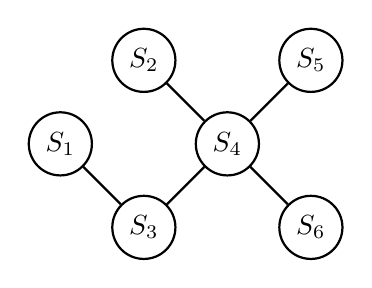
\begin{tikzpicture}[node distance={15mm}, thick, main/.style = {draw, circle}]
		\node[main] (1) {$S_1$}; 
		\node[main] (2) [above right of=1] {$S_2$};
		\node[main] (3) [below right of=1] {$S_3$}; 
		\node[main] (4) [above right of=3] {$S_4$};
		\node[main] (5) [above right of=4] {$S_5$}; 
		\node[main] (6) [below right of=4] {$S_6$};
		\draw (2) -- (4);
		\draw (1) -- (3);
		\draw (3) -- (4);
		\draw (4) -- (5);
		\draw (4) -- (6);
	\end{tikzpicture} 
\end{document}